\documentclass[tikz,border=2mm]{standalone}
\usepackage{amsmath,amssymb}
\usepackage[T1]{fontenc}
\usepackage{lmodern}
\usetikzlibrary{arrows.meta,calc,positioning,decorations.pathreplacing,shapes.geometric,fit}

% Requested muted palette
\definecolor{mistyblue}{HTML}{A3BFD9}
\definecolor{slateblue}{HTML}{7A90B2}
\definecolor{sagegreen}{HTML}{A3BFA3}
\definecolor{dustyteal}{HTML}{6E8B8B}
\definecolor{softgray}{HTML}{D8D8D8}
\definecolor{deepmutedblue}{HTML}{4A5A6A}

% Backward-compatible aliases used throughout the figure
\colorlet{deepblue}{deepmutedblue}
\colorlet{lineblue}{slateblue}
\colorlet{barblue}{mistyblue}
\colorlet{darkgreen}{dustyteal}
\colorlet{softgreen}{softgray}
\colorlet{purple}{slateblue}
\colorlet{mutedorange}{sagegreen}
\colorlet{brownline}{deepmutedblue}
\colorlet{brownfill}{softgray}
\colorlet{lightblue}{softgray}
\colorlet{grayline}{softgray}
\colorlet{darkred}{deepmutedblue}

\newcommand{\panel}[4]{\draw[lineblue, rounded corners=2pt, line width=0.8pt] (#1,#2) rectangle ++(#3,#4);}
\newcommand{\numcircle}[3]{\node[circle, fill=deepblue, text=white, inner sep=1.5pt, minimum size=0.47cm, font=\bfseries\small] at (#1,#2) {#3};}
\newcommand{\sq}[5]{\node[draw=none, rounded corners=1.4pt, fill=#4, text=white, minimum width=0.46cm, minimum height=0.46cm, inner sep=0pt, font=\bfseries\small] at (#1,#2) {#5};}
\newcommand{\tinysq}[3]{\draw[fill=#3, draw=#3, rounded corners=1pt] (#1,#2) rectangle ++(0.30,0.30);}

\begin{document}
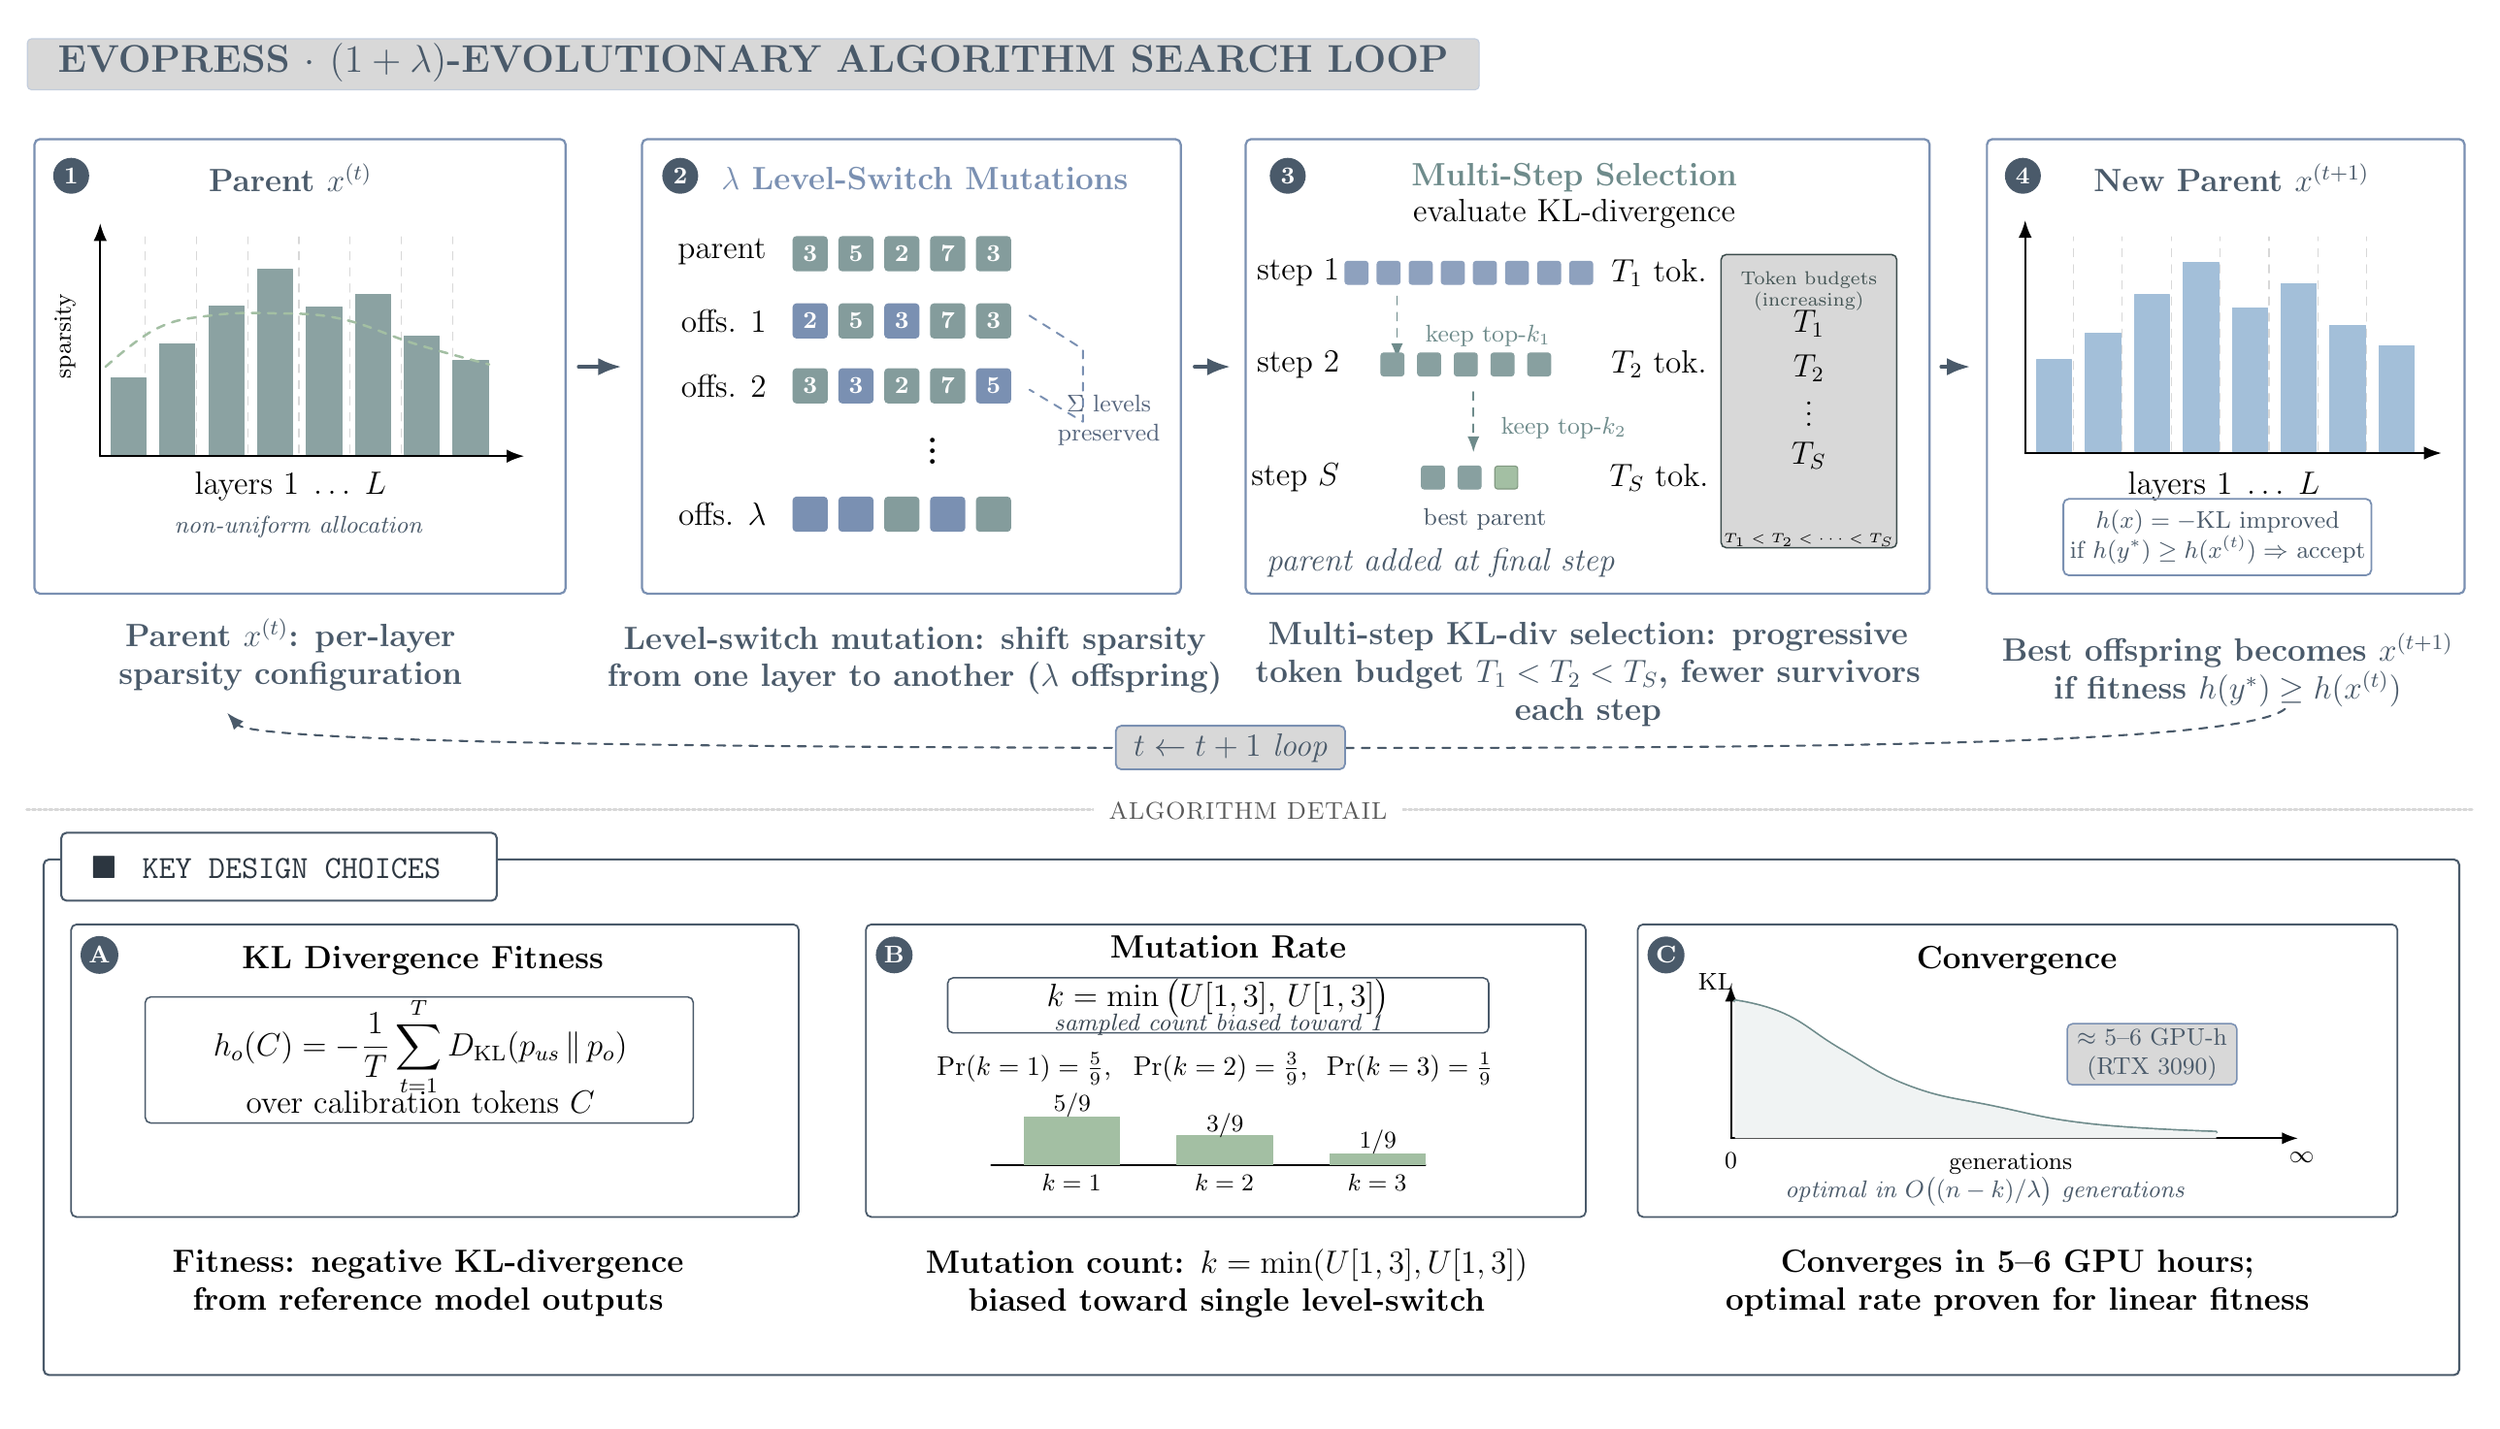
\begin{tikzpicture}[x=1cm,y=1cm,>=Latex,line cap=round,line join=round]
\path[use as bounding box] (0,0) rectangle (32,18);
\fill[white] (0,0) rectangle (32,18);

% ------------------------------------------------------------------
% Title
% ------------------------------------------------------------------
\node[anchor=north west, draw=lineblue!45, fill=lightblue, rounded corners=1.5pt,
      inner xsep=0.40cm, inner ysep=0.10cm,
      text=deepblue, font=\bfseries\Large\scshape, text height=0.34cm]
      at (0.00,17.85) {EVOPRESS $\cdot$ $(1+\lambda)$-EVOLUTIONARY ALGORITHM SEARCH LOOP};

% ------------------------------------------------------------------
% Top row panels
% ------------------------------------------------------------------
\panel{0.10}{10.58}{6.95}{5.95}
\panel{8.05}{10.58}{7.05}{5.95}
\panel{15.95}{10.58}{8.95}{5.95}
\panel{25.65}{10.58}{6.25}{5.95}

% arrows between panels
\draw[-Latex, line width=1.25pt, deepblue] (7.22,13.55) -- (7.78,13.55);
\draw[-Latex, line width=1.25pt, deepblue] (15.28,13.55) -- (15.75,13.55);
\draw[-Latex, line width=1.25pt, deepblue] (25.05,13.55) -- (25.43,13.55);

% ------------------------------------------------------------------
% Panel 1: Parent chart
% ------------------------------------------------------------------
\numcircle{0.58}{16.05}{1}
\node[font=\bfseries\large, text=deepblue] at (3.45,16.02) {Parent $x^{(t)}$};

% chart area
\begin{scope}
\coordinate (A) at (0.96,12.38);
\draw[-Latex, line width=0.8pt] (A) -- ++(5.55,0);
\draw[-Latex, line width=0.8pt] (A) -- ++(0,3.05);
\node[rotate=90, font=\small] at (0.50,13.95) {sparsity};
\node[font=\large] at (3.45,11.98) {layers $1\;\ldots\;L$};
\foreach \x in {1.55,2.22,2.89,3.56,4.23,4.90,5.57} {
  \draw[grayline, dashed, line width=0.45pt] (\x,12.42) -- (\x,15.25);
}
\foreach \x/\h in {1.10/1.00,1.74/1.45,2.38/1.95,3.02/2.42,3.66/1.93,4.30/2.10,4.94/1.55,5.58/1.23}{
  \draw[fill=darkgreen!80, draw=darkgreen!80] (\x,12.40) rectangle ++(0.46,\h);
}
\draw[mutedorange, dashed, line width=0.9pt]
  plot[smooth,tension=0.7] coordinates {(1.03,13.55) (1.70,14.05) (2.40,14.22) (3.20,14.25) (4.10,14.18) (5.08,13.85) (6.05,13.58)};
\node[font=\itshape\small, text=deepblue] at (3.55,11.45) {non-uniform allocation};
\end{scope}

\node[align=center, font=\bfseries\large, text=deepblue] at (3.45,9.78)
  {Parent $x^{(t)}$: per-layer\\sparsity configuration};

% ------------------------------------------------------------------
% Panel 2: Level-switch mutations
% ------------------------------------------------------------------
\numcircle{8.55}{16.05}{2}
\node[font=\bfseries\large, text=purple] at (11.75,16.02) {$\lambda$ Level-Switch Mutations};

\node[anchor=east, font=\large] at (9.80,15.05) {parent};
\node[anchor=east, font=\large] at (9.80,14.15) {offs. 1};
\node[anchor=east, font=\large] at (9.80,13.30) {offs. 2};
\node[anchor=east, font=\large] at (9.80,11.62) {offs. $\lambda$};
\node[font=\bfseries\large] at (11.85,12.55) {$\vdots$};

% rows of level squares
\foreach \x/\v in {10.25/3,10.85/5,11.45/2,12.05/7,12.65/3}{\sq{\x}{15.03}{0.48}{darkgreen!85}{\v}}
\foreach \x/\v/\c in {10.25/2/purple,10.85/5/darkgreen!85,11.45/3/purple,12.05/7/darkgreen!85,12.65/3/darkgreen!85}{\sq{\x}{14.15}{0.48}{\c}{\v}}
\foreach \x/\v/\c in {10.25/3/darkgreen!85,10.85/3/purple,11.45/2/darkgreen!85,12.05/7/darkgreen!85,12.65/5/purple}{\sq{\x}{13.30}{0.48}{\c}{\v}}
\foreach \x/\c in {10.25/purple,10.85/purple,11.45/darkgreen!85,12.05/purple,12.65/darkgreen!85}{\sq{\x}{11.62}{0.48}{\c}{}}

% side brace and text
\draw[purple, dashed, line width=0.7pt] (13.12,14.22) -- (13.82,13.78) -- (13.82,12.83) -- (13.12,13.25);
\node[align=center, text=purple!70!black, font=\small] at (14.16,12.85) {$\Sigma$ levels\\preserved};

\node[align=center, font=\bfseries\large, text=deepblue] at (11.62,9.70)
  {Level-switch mutation: shift sparsity\\from one layer to another ($\lambda$ offspring)};

% ------------------------------------------------------------------
% Panel 3: Multi-step selection
% ------------------------------------------------------------------
\numcircle{16.50}{16.05}{3}
\node[font=\bfseries\large, text=darkgreen] at (20.25,16.03) {Multi-Step Selection};
\node[font=\large] at (20.25,15.55) {evaluate KL-divergence};

\node[anchor=east, font=\large] at (17.30,14.78) {step $1$};
\foreach \i in {0,...,7}{\tinysq{17.25+0.42*\i}{14.63}{purple!85}}
\node[font=\large] at (21.36,14.78) {$T_1$ tok.};
\draw[darkgreen, dashed, -Latex, line width=0.65pt] (17.93,14.47) -- (17.93,13.65);
\node[anchor=west, font=\small, text=darkgreen] at (18.18,13.95) {keep top-$k_1$};

\node[anchor=east, font=\large] at (17.30,13.58) {step $2$};
\foreach \i in {0,...,4}{\tinysq{17.72+0.48*\i}{13.43}{darkgreen!82}}
\node[font=\large] at (21.36,13.58) {$T_2$ tok.};
\draw[darkgreen, dashed, -Latex, line width=0.65pt] (18.93,13.22) -- (18.93,12.43);
\node[anchor=west, font=\small, text=darkgreen] at (19.17,12.75) {keep top-$k_2$};

\node[anchor=east, font=\large] at (17.30,12.10) {step $S$};
\tinysq{18.25}{11.95}{darkgreen!82}
\tinysq{18.73}{11.95}{darkgreen!82}
\draw[fill=mutedorange, draw=mutedorange!80!black, rounded corners=1pt] (19.21,11.95) rectangle ++(0.30,0.30);
\node[font=\small, text=darkred] at (19.08,11.55) {best parent};
\node[font=\itshape\large, text=darkred] at (18.50,10.98) {parent added at final step};
\node[font=\large] at (21.36,12.10) {$T_S$ tok.};

% token budget box
\draw[darkgreen!55!black, fill=softgreen, rounded corners=2pt, line width=0.55pt] (22.17,11.18) rectangle (24.47,15.02);
\node[align=center, font=\scriptsize, text=darkgreen!60!black] at (23.32,14.54) {Token budgets\\(increasing)};
\node[align=center, font=\large] at (23.32,13.25) {$T_1$\\[0.10cm]$T_2$\\[0.01cm]$\vdots$\\[0.01cm]$T_S$};
\node[font=\tiny] at (23.32,11.28) {$T_1<T_2<\cdots<T_S$};

\node[align=center, font=\bfseries\large, text=deepblue] at (20.43,9.52)
  {Multi-step KL-div selection: progressive\\token budget $T_1<T_2<T_S$, fewer survivors\\each step};

% ------------------------------------------------------------------
% Panel 4: New parent chart
% ------------------------------------------------------------------
\numcircle{26.12}{16.05}{4}
\node[font=\bfseries\large, text=deepblue] at (28.85,16.02) {New Parent $x^{(t+1)}$};

\begin{scope}
\coordinate (B) at (26.15,12.42);
\draw[-Latex, line width=0.8pt] (B) -- ++(5.45,0);
\draw[-Latex, line width=0.8pt] (B) -- ++(0,3.05);
\node[font=\large] at (28.75,11.98) {layers $1\;\ldots\;L$};
\foreach \x in {26.78,27.42,28.06,28.70,29.34,29.98,30.62}{
  \draw[grayline, dashed, line width=0.45pt] (\x,12.46) -- (\x,15.25);
}
\foreach \x/\h in {26.30/1.20,26.94/1.55,27.58/2.05,28.22/2.48,28.86/1.88,29.50/2.20,30.14/1.65,30.78/1.38}{
  \draw[fill=barblue, draw=barblue] (\x,12.44) rectangle ++(0.46,\h);
}
\end{scope}

\draw[lineblue, rounded corners=2pt, line width=0.65pt] (26.65,10.82) rectangle (30.68,11.82);
\node[align=center, font=\small, text=deepblue] at (28.67,11.32)
  {$h(x)=-\mathrm{KL}$ improved\\if $h(y^*)\geq h(x^{(t)})\Rightarrow$ accept};

\node[align=center, font=\bfseries\large, text=deepblue] at (28.80,9.58)
  {Best offspring becomes $x^{(t+1)}$\\if fitness $h(y^*)\geq h(x^{(t)})$};

% ------------------------------------------------------------------
% Dashed loop arrow and separator
% ------------------------------------------------------------------
\draw[deepblue, dashed, line width=0.75pt, -Latex]
  (29.55,9.07) .. controls (28.9,8.55) and (22.0,8.56) .. (16.15,8.56)
              .. controls (10.8,8.56) and (3.0,8.60) .. (2.62,9.02);
\draw[lineblue, rounded corners=2pt, fill=lightblue, line width=0.65pt] (14.25,8.28) rectangle (17.25,8.85);
\node[font=\large\itshape, text=deepblue] at (15.75,8.56) {$t\leftarrow t+1$ loop};

\draw[densely dotted, line width=1.1pt, grayline] (0.0,7.75) -- (32.0,7.75);
\node[fill=white, inner xsep=0.20cm, font=\small\scshape, text=black!65] at (15.98,7.73) {ALGORITHM DETAIL};

% ------------------------------------------------------------------
% Bottom: key design choices
% ------------------------------------------------------------------
\draw[brownline, rounded corners=2pt, line width=0.75pt] (0.22,0.35) rectangle (31.83,7.10);
\draw[brownline, rounded corners=2pt, fill=white, line width=0.75pt] (0.45,6.56) rectangle (6.15,7.45);
\node[anchor=west, font=\bfseries\large\ttfamily, text=brownline!60!black] at (0.72,7.00)
  {$\blacksquare$\; KEY DESIGN CHOICES};

% Detail panel A
\draw[brownline, rounded corners=2pt, line width=0.65pt] (0.58,2.42) rectangle (10.10,6.25);
\node[circle, fill=brownline, text=white, inner sep=1.4pt, minimum size=0.47cm, font=\bfseries\small] at (0.95,5.85) {A};
\node[font=\bfseries\large] at (5.18,5.78) {KL Divergence Fitness};
\draw[brownline, rounded corners=2pt, line width=0.55pt] (1.55,3.65) rectangle (8.72,5.30);
\node[font=\large] at (5.15,4.65) {$h_o(C)=-\dfrac{1}{T}\displaystyle\sum_{t=1}^{T}D_{\mathrm{KL}}\!\left(p_{us}\,\middle\|\,p_o\right)$};
\node[font=\large] at (5.15,3.93) {over calibration tokens $C$};
\node[align=center, font=\bfseries\large] at (5.25,1.55) {Fitness: negative KL-divergence\\from reference model outputs};

% Detail panel B
\draw[brownline, rounded corners=2pt, line width=0.65pt] (10.98,2.42) rectangle (20.40,6.25);
\node[circle, fill=brownline, text=white, inner sep=1.4pt, minimum size=0.47cm, font=\bfseries\small] at (11.35,5.85) {B};
\node[font=\bfseries\large] at (15.72,5.96) {Mutation Rate};
\draw[brownline, rounded corners=2pt, line width=0.55pt] (12.05,4.83) rectangle (19.13,5.55);
\node[font=\large] at (15.59,5.28) {$k=\min\big(U[1,3],\,U[1,3]\big)$};
\node[font=\itshape\small, text=brownline!75!black] at (15.59,4.94) {sampled count biased toward 1};
\node[font=\normalsize] at (13.05,4.36) {$\Pr(k=1)=\frac{5}{9}$,};
\node[font=\normalsize] at (15.62,4.36) {$\Pr(k=2)=\frac{3}{9}$,};
\node[font=\normalsize] at (18.10,4.36) {$\Pr(k=3)=\frac{1}{9}$};
\draw[black, line width=0.65pt] (12.62,3.10) -- (18.30,3.10);
\foreach \x/\h/\lab/\frac in {13.05/0.63/$k=1$/5/9,15.05/0.38/$k=2$/3/9,17.05/0.15/$k=3$/1/9}{
  \draw[fill=mutedorange, draw=mutedorange] (\x,3.10) rectangle ++(1.25,\h);
  \node[font=\small] at (\x+0.62,2.87) {\lab};
}
\node[font=\small] at (13.68,3.88) {$5/9$};
\node[font=\small] at (15.68,3.62) {$3/9$};
\node[font=\small] at (17.68,3.40) {$1/9$};
\node[align=center, font=\bfseries\large] at (15.70,1.55) {Mutation count: $k=\min(U[1,3],U[1,3])$\\biased toward single level-switch};

% Detail panel C
\draw[brownline, rounded corners=2pt, line width=0.65pt] (21.08,2.42) rectangle (31.02,6.25);
\node[circle, fill=brownline, text=white, inner sep=1.4pt, minimum size=0.47cm, font=\bfseries\small] at (21.45,5.85) {C};
\node[font=\bfseries\large] at (26.04,5.78) {Convergence};
\draw[->, line width=0.65pt] (22.30,3.45) -- (29.72,3.45);
\draw[->, line width=0.65pt] (22.30,3.45) -- (22.30,5.45);
\node[font=\small] at (22.10,5.50) {KL};
\node[font=\small] at (22.30,3.15) {0};
\node[font=\small] at (29.77,3.20) {$\infty$};
\node[font=\small] at (25.96,3.12) {generations};
\draw[darkgreen, line width=1.2pt]
  plot[smooth,tension=0.75] coordinates {(22.35,5.25) (23.00,5.07) (23.75,4.60) (24.65,4.12) (25.75,3.86) (27.00,3.63) (28.65,3.53)};
\fill[darkgreen!10] (22.35,3.45) -- plot[smooth,tension=0.75] coordinates {(22.35,5.25) (23.00,5.07) (23.75,4.60) (24.65,4.12) (25.75,3.86) (27.00,3.63) (28.65,3.53)} -- (28.65,3.45) -- cycle;
\draw[lineblue, rounded corners=2pt, fill=lightblue, line width=0.55pt] (26.70,4.15) rectangle (28.92,4.95);
\node[align=center, font=\small, text=deepblue] at (27.81,4.55) {$\approx$ 5--6 GPU-h\\(RTX 3090)};
\node[font=\itshape\small, text=deepblue] at (25.62,2.75) {optimal in $O\big((n-k)/\lambda\big)$ generations};
\node[align=center, font=\bfseries\large] at (26.05,1.55) {Converges in 5--6 GPU hours;\\optimal rate proven for linear fitness};

\end{tikzpicture}
\end{document}
